\documentclass[pdf]{beamer}
\usepackage[utf8]{inputenc}
\mode<presentation>{
	\usetheme[block=fill,]{metropolis}
}

\usepackage{booktabs}
\usepackage{tabularx}
\usepackage{hyperref}
\usepackage{appendixnumberbeamer}
\usepackage{caption}
\usepackage{graphicx}
\usepackage{multirow}
\usepackage{bm}
\usepackage{amsfonts}
\usepackage{amsmath}
\usepackage{subcaption}

\setbeamertemplate{itemize subitem}{\tiny\raise1.5pt\hbox{\donotcoloroutermaths$\blacktriangleright$}}

\graphicspath{{images/}}

\begin{document}

	\begin{frame}[plain, noframenumbering]
		\title{Deep Learning for Portfolio Optimization}
		\author{Reference: \url{https://jfds.pm-research.com/content/2/4/8}}
		\date{Implemented from scratch by Marco Lazzarin}
		\titlepage
	\end{frame}

	%\setbeamertemplate{itemize item}{\alert{$\bullet$}}

	\setbeamertemplate{itemize item}{\color{black}$\bullet$}

	\begin{frame}{Asset allocation}
		Let $P^t$ be the total equity at time $t$ and consider $n$ securities.
		\begin{itemize}
			\item $p_i^t$: counter value of asset $i$ at time $t$.
			\item $\sum_i p_i^t = P^t$.
			\item $w_i^t$: weight of asset $i$ at time $t$.
			\item $w_i^t = p_i^t / P^t$.
			\item $\sum_i w_i^t = 1$ .
		\end{itemize}
		\textcolor{blue}{Goal:} optimize $\{ w_i^t \}$ to obtain the \alert{best} possible portfolio.
	\end{frame}

	\begin{frame}{Historical data}
		Consider four different ETFs:

		\centering
		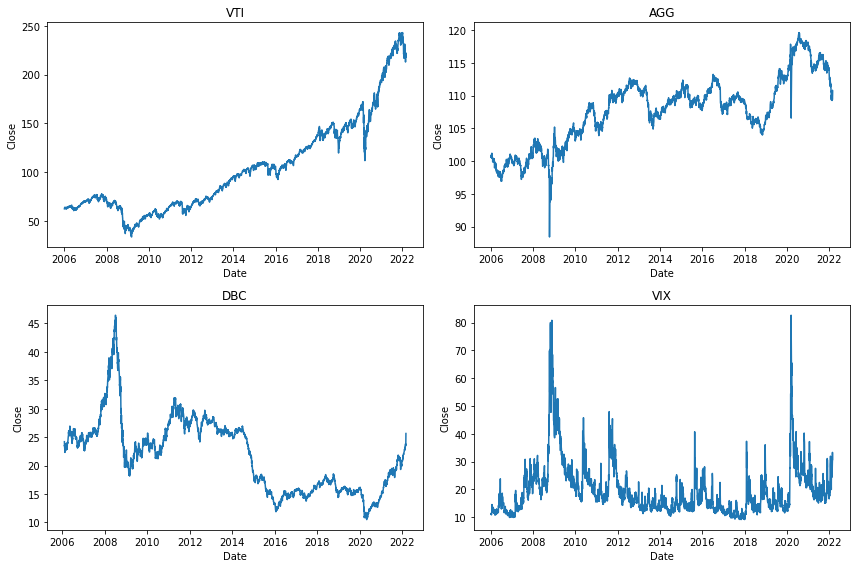
\includegraphics[width=0.6\textwidth]{historical_data.png}

		\raggedright
		Let $x_i^t$ be the close price of asset $i$ at time $t$.
		\begin{itemize}
			\item $r_i^{t+1} = x_i^{t+1}/x_i^t - 1$: return of asset $i$ at time $t+1$.
			\item $R^{t+1} = \sum_i w_i^t r_i^{t+1}$: total return at time $t+1$.
		\end{itemize}
	\end{frame}

	\begin{frame}{Reallocation strategy}
		Impose fixed weights $\{ w_i^t \} = W_i$ every $T$ time steps.
		\begin{itemize}
			\item $w_i^t = W_i \quad \forall t = kT, k \in \mathbb{N}$.
			\item Otherwise $w_i^{t+1} = w_i^t (r_i^{t+1} + 1) / \sum_k w_k^t (r_k^{t+1} + 1)$.
		\end{itemize}

		\centering
		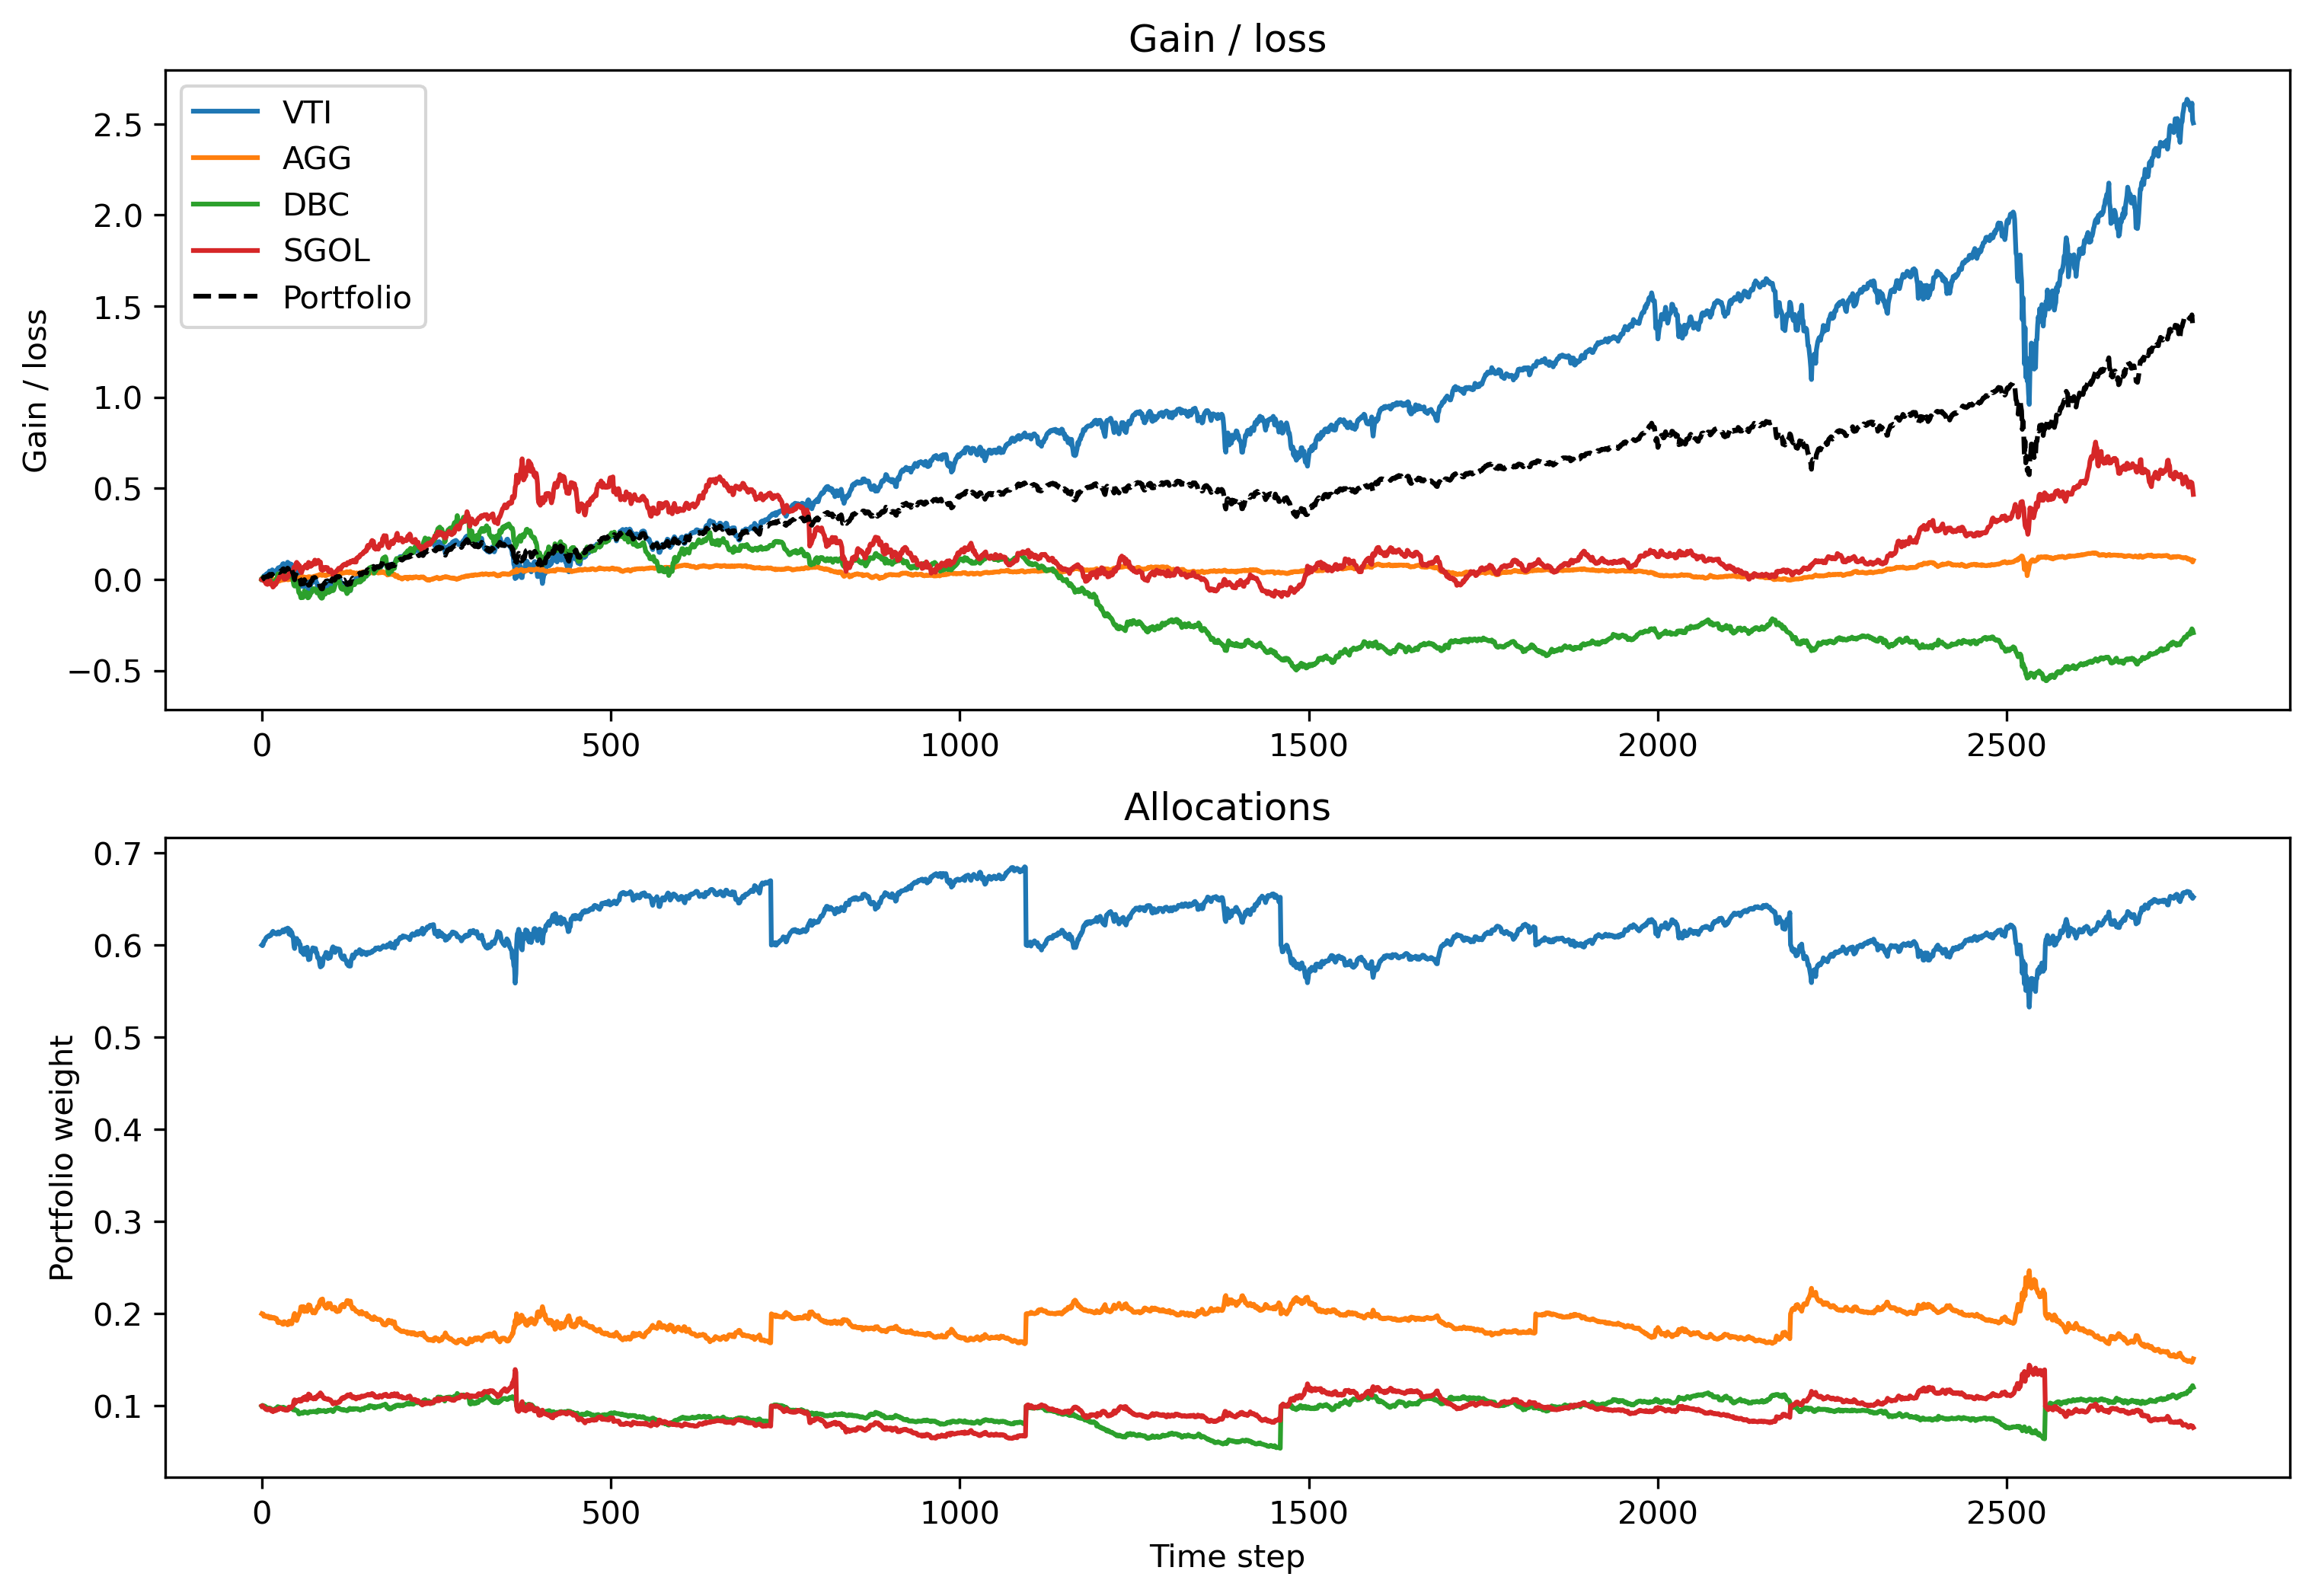
\includegraphics[width=0.75\textwidth]{reallocation_strategy.png}
	\end{frame}

	\begin{frame}{Deep learning optimization}
		Use a deep learning model to predict portfolio weights $\{ w_i^t \}$.
		
		\vfill
		\centering
		\includegraphics[width=\textwidth]{DeepLearningOptimizer.png}
	\end{frame}

	\begin{frame}{How to train the model?}
		\textcolor{blue}{Maximize the Sharpe ratio:}
		$$ L = \frac{E [ R^t ]}{\sqrt{Var [ R^t ]}} $$
		where $E[ R^t ]$ and $Var [ R^t ]$ are the first two moments of the returns.

		Overview:
		\begin{itemize}
			\item Input data $x_i^t$ of shape (batch size, time steps, features).
			\item Model $\to$ weights $w_i^t$ of shape (batch size, time steps, assets).
			\item Compute distribution of returns $R^t$ of shape (batch size, time steps - 1).
			\item Compute Sharpe ratio and run Adam optimizer.
		\end{itemize}

	\end{frame}

	\begin{frame}{Results}
		\centering
		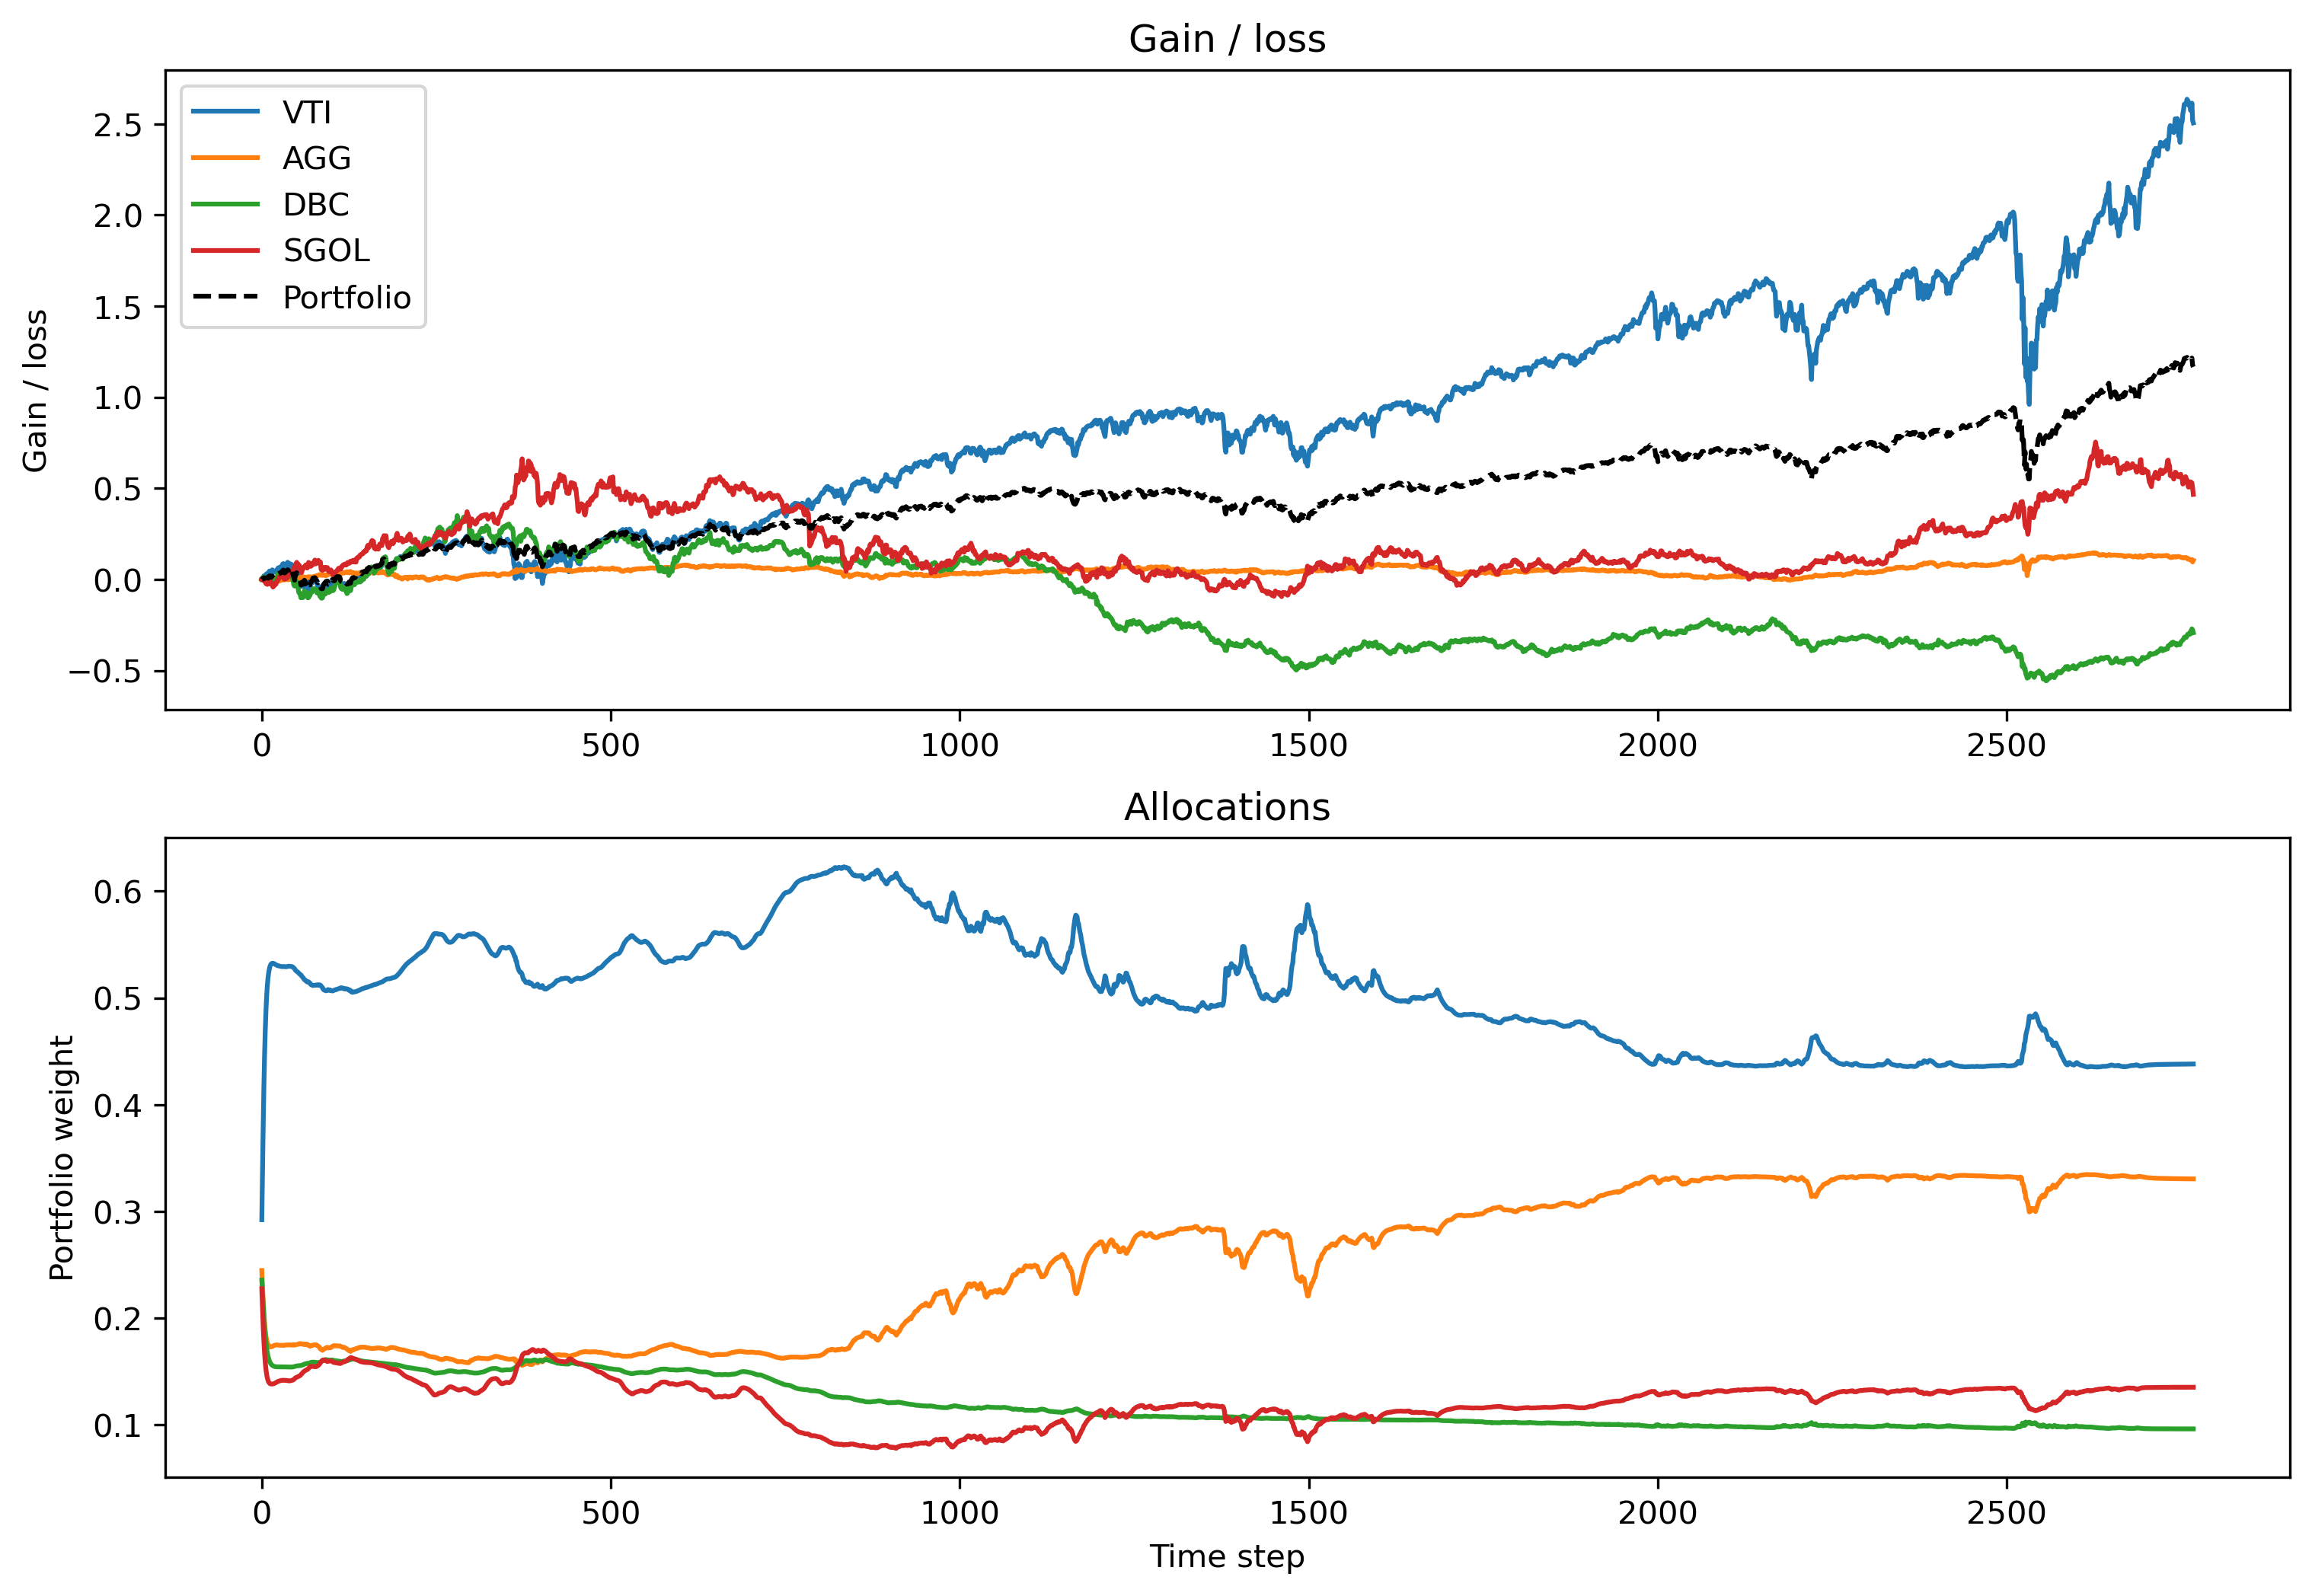
\includegraphics[width=\textwidth]{deep_learning_optimization.png}
	\end{frame}

	\begin{frame}{Sensitivity to hyperparameters}
		\alert{Problem:} if I change architecture $\to$ very different allocations!\\
		Allocation of VTI with different architectures:
		
		\vfill
		\centering
		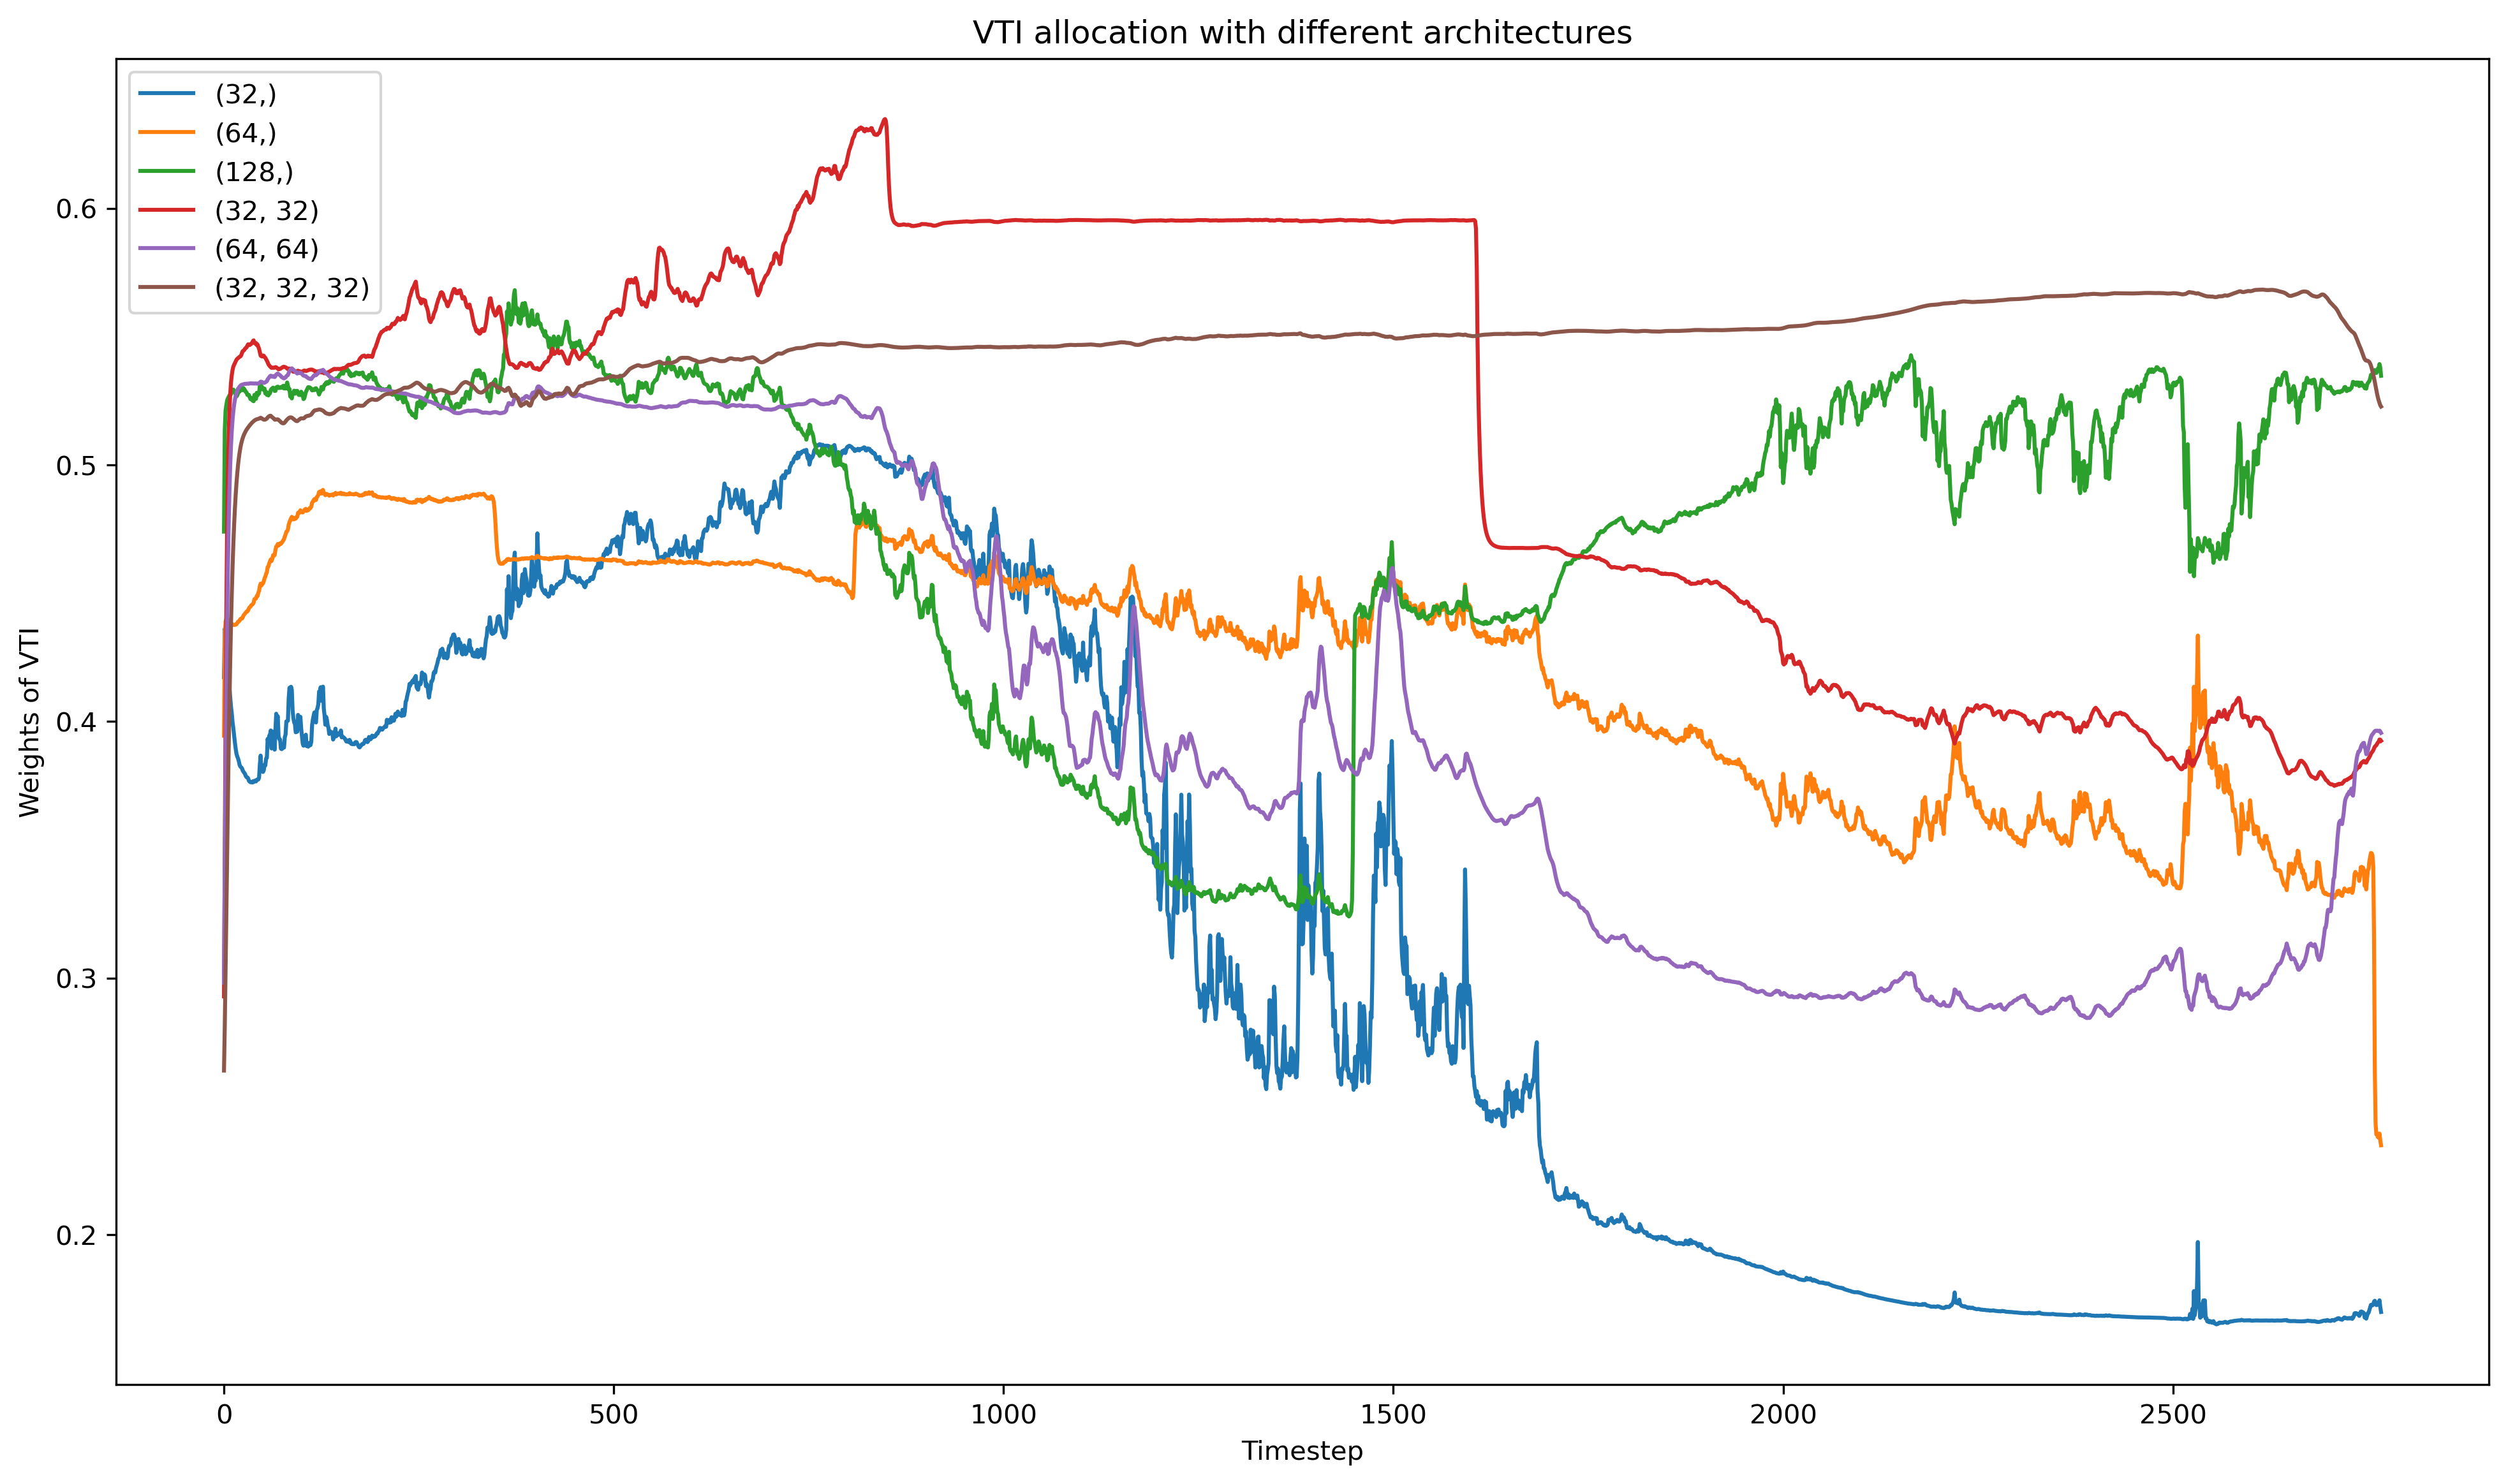
\includegraphics[width=\textwidth]{hyperscan.png}
	\end{frame}

\end{document}